\documentclass[a4paper,12pt]{article}

\usepackage{color}
\usepackage{amsmath, amssymb}
\usepackage{verbatim}
\usepackage{tikz} 
\usetikzlibrary{shapes}
\usetikzlibrary{arrows}
\usetikzlibrary{positioning}
\usetikzlibrary{patterns}
\usetikzlibrary{calc}
\usetikzlibrary{shapes.geometric}
\usetikzlibrary{backgrounds,calc,shadings,shapes.arrows,shapes.symbols,shadows}

\begin{document}
\title{My First Document}
\author{SJAbd}
\date{\today}
\maketitle


\setlength{\unitlength}{5cm}
\begin{picture}(1,1)
\put(0,0){\line(0,1){1}}
\put(0,0){\line(1,0){1}}
\put(0,0){\line(1,1){1}}
\put(0,0){\line(1,2){.5}}
\put(0,0){\line(1,3){.3333}}
\put(0,0){\line(1,4){.25}}
\put(0,0){\line(1,5){.2}}
\put(0,0){\line(1,6){.1667}}
\put(0,0){\line(2,1){1}}
\put(0,0){\line(2,3){.6667}}
\put(0,0){\line(2,5){.4}}
\put(0,0){\line(3,1){1}}
\put(0,0){\line(3,2){1}}
\put(0,0){\line(3,4){.75}}
\put(0,0){\line(3,5){.6}}
\put(0,0){\line(4,1){1}}
\put(0,0){\line(4,3){1}}
\put(0,0){\line(4,5){.8}}
\put(0,0){\line(5,1){1}}
\put(0,0){\line(5,2){1}}
\put(0,0){\line(5,3){1}}
\put(0,0){\line(5,4){1}}
\put(0,0){\line(5,6){.8333}}
\put(0,0){\line(6,1){1}}
\put(0,0){\line(6,5){1}}
\end{picture}



\setlength{\unitlength}{0.75mm}
\begin{picture}(60,40)
\put(30,20){\vector(1,0){30}}
\put(30,20){\vector(4,1){20}}
\put(30,20){\vector(3,1){25}}
\put(30,20){\vector(2,1){30}}
\put(30,20){\vector(1,2){10}}
\thicklines
\put(30,20){\vector(-4,1){30}}
\put(30,20){\vector(-1,4){5}}
\thinlines
\put(30,20){\vector(-1,-1){5}}
\put(30,20){\vector(-1,-4){5}}
\end{picture}





\setlength{\unitlength}{1mm}
\begin{picture}(60, 40)
\put(20,30){\circle{1}}
\put(20,30){\circle{2}}
\put(20,30){\circle{4}}
\put(20,30){\circle{8}}
\put(20,30){\circle{16}}
\put(20,30){\circle{32}}
\put(40,30){\circle{1}}
\put(40,30){\circle{2}}
\put(40,30){\circle{3}}
\put(40,30){\circle{4}}
\put(40,30){\circle{5}}
\put(40,30){\circle{6}}
\put(40,30){\circle{7}}
\put(40,30){\circle{8}}
\put(40,30){\circle{9}}
\put(40,30){\circle{10}}
\put(40,30){\circle{11}}
\put(40,30){\circle{12}}
\put(40,30){\circle{13}}
\put(40,30){\circle{14}}
\put(15,10){\circle*{1}}
\put(20,10){\circle*{2}}
\put(25,10){\circle*{3}}
\put(30,10){\circle*{4}}
\put(35,10){\circle*{5}}
\end{picture}





\setlength{\unitlength}{0.8cm}
\begin{picture}(6,5)
\thicklines
\put(1,0.5){\line(2,1){3}}
\put(4,2){\line(-2,1){2}}
\put(2,3){\line(-2,-5){1}}
\put(0.7,0.3){$A$}
\put(4.05,1.9){$B$}
\put(1.7,2.95){$C$}
\put(3.1,2.5){$a$}
\put(1.3,1.7){$b$}
\put(2.5,1.05){$c$}
\put(0.3,4){$F=
\sqrt{s(s-a)(s-b)(s-c)}$}
\put(3.5,0.4){$\displaystyle
s:=\frac{a+b+c}{2}$}
\end{picture}



\setlength{\unitlength}{2mm}
\begin{picture}(30,20)
\linethickness{0.075mm}
\multiput(0,0)(1,0){26}%
{\line(0,1){20}}
\multiput(0,0)(0,1){21}%
{\line(1,0){25}}
\linethickness{0.15mm}
\multiput(0,0)(5,0){6}%
{\line(0,1){20}}
\multiput(0,0)(0,5){5}%
{\line(1,0){25}}
\linethickness{0.3mm}
\multiput(5,0)(10,0){2}%
{\line(0,1){20}}
\multiput(0,5)(0,10){2}%
{\line(1,0){25}}
\end{picture}





\setlength{\unitlength}{0.75cm}
\begin{picture}(6,4)
\linethickness{0.075mm}
\multiput(0,0)(1,0){7}%
{\line(0,1){4}}
\multiput(0,0)(0,1){5}%
{\line(1,0){6}}
\thicklines
\put(2,3){\oval(3,1.8)}
\thinlines
\put(3,2){\oval(3,1.8)}
\thicklines
\put(2,1){\oval(3,1.8)[tl]}
\put(4,1){\oval(3,1.8)[b]}
\put(4,3){\oval(3,1.8)[r]}
\put(3,1.5){\oval(1.8,0.4)}
\end{picture}




\setlength{\unitlength}{0.5mm}
\begin{picture}(120,168)
\newsavebox{\foldera}
\savebox{\foldera}
(40,32)[bl]{% definition
	\multiput(0,0)(0,28){2}{\line(1,0){40}}
	\multiput(0,0)(40,0){2}{\line(0,1){28}}
	\put(1,28){\oval(2,2)[tl]}
	\put(1,29){\line(1,0){5}}
	\put(9,29){\oval(6,6)[tl]}
	\put(9,32){\line(1,0){8}}
	\put(17,29){\oval(6,6)[tr]}
	%\put(20,29){\line(1,0){19}}
	%\put(39,28){\oval(2,2)[tr]}
}
\newsavebox{\folderb}
\savebox{\folderb}
(40,32)[l]{% definition
	\put(0,14){\line(1,0){8}}
	\put(8,0){\usebox{\foldera}}
}
\put(34,26){\line(0,1){102}}
\put(14,128){\usebox{\foldera}}
\multiput(34,86)(0,-37){3}{\usebox{\folderb}}
\end{picture}




\setlength{\unitlength}{1cm}
\begin{picture}(4.3,3.6)(-2.5,-0.25)
\put(-2,0){\vector(1,0){4.4}}
\put(2.45,-.05){$x$}
\put(0,0){\vector(0,1){3.2}}
\put(0,3.35){\makebox(0,0){$y$}}
\qbezier(0.0,0.0)(1.2384,0.0)
(2.0,2.7622)
\qbezier(0.0,0.0)(-1.2384,0.0)
(-2.0,2.7622)
\linethickness{.075mm}
\multiput(-2,0)(1,0){5}
{\line(0,1){3}}
\multiput(-2,0)(0,1){4}
{\line(1,0){4}}
\linethickness{.2mm}
\put( .3,.12763){\line(1,0){.4}}
\put(.5,-.07237){\line(0,1){.4}}
\put(-.7,.12763){\line(1,0){.4}}
\put(-.5,-.07237){\line(0,1){.4}}
\put(.8,.54308){\line(1,0){.4}}
\put(1,.34308){\line(0,1){.4}}
\put(-1.2,.54308){\line(1,0){.4}}
\put(-1,.34308){\line(0,1){.4}}
\put(1.3,1.35241){\line(1,0){.4}}
\put(1.5,1.15241){\line(0,1){.4}}
\put(-1.7,1.35241){\line(1,0){.4}}
\put(-1.5,1.15241){\line(0,1){.4}}
\put(-2.5,-0.25){\circle*{0.2}}
\end{picture}





\setlength{\unitlength}{0.8cm}
\begin{picture}(6,4)(-3,-2)
\put(-2.5,0){\vector(1,0){5}}
\put(2.7,-0.1){$\chi$}
\put(0,-1.5){\vector(0,1){3}}
\multiput(-2.5,1)(0.4,0){13}
{\line(1,0){0.2}}
\multiput(-2.5,-1)(0.4,0){13}
{\line(1,0){0.2}}
\put(0.2,1.4)
{$\beta=v/c=\tanh\chi$}
\qbezier(0,0)(0.8853,0.8853)
(2,0.9640)
\qbezier(0,0)(-0.8853,-0.8853)
(-2,-0.9640)
\put(-3,-2){\circle*{0.2}}
\end{picture}





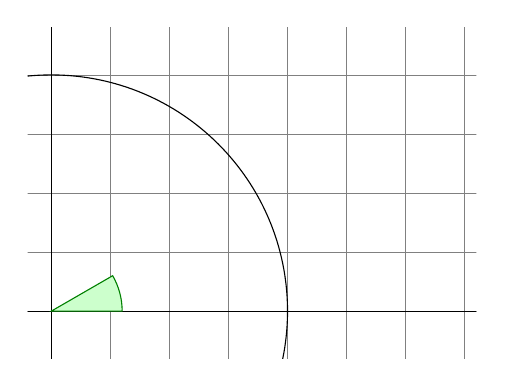
\begin{tikzpicture}[scale=3]
\clip (-0.1,-0.2)
rectangle (1.8,1.2);
\draw[step=.25cm,gray,very thin]
(-1.4,-1.4) grid (3.4,3.4);
\draw (-1.5,0) -- (2.5,0);
\draw (0,-1.5) -- (0,1.5);
\draw (0,0) circle (1cm);
\filldraw[fill=green!20!white,
draw=green!50!black]
(0,0) -- (3mm,0mm)
arc (0:30:3mm) -- cycle;
\end{tikzpicture}




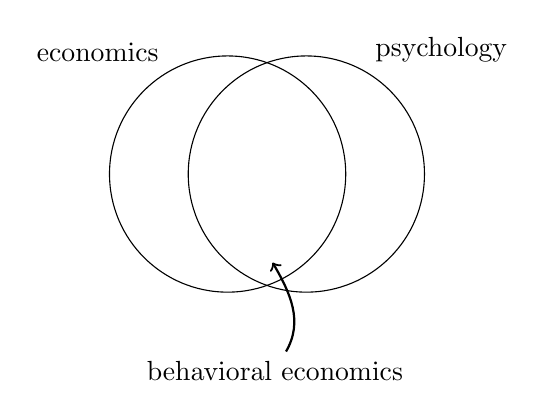
\begin{tikzpicture}
\node[circle,draw,
minimum size=3cm,
label=120:{economics}]
at (0,0) {};
\node[circle,draw,
minimum size=3cm,
label=60:{psychology}]
at (1,0) {};
\node (i) at (0.5,-1) {};
\node at (0.6,-2.5)
{behavioral economics}
edge[->,thick,
out=60,in=-60] (i);
\end{tikzpicture}





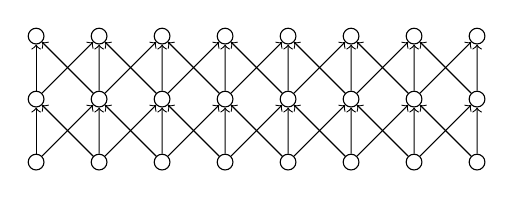
\begin{tikzpicture}[scale=0.8]
\tikzstyle{v}=[circle, minimum size=2mm,inner sep=0pt,draw]
\foreach \i in {1,...,8}
\foreach \j in {1,...,3}
\node[v]
(G-\i-\j) at (\i,\j) {};
\foreach \i in {1,...,8}
\foreach \j/\o in {1/2,2/3}
\draw[->]
(G-\i-\j) -- (G-\i-\o);
\foreach \i/\n in
{1/2,2/3,3/4,4/5,5/6,6/7,7/8}
\foreach \j/\o in {1/2,2/3} {
\draw[->] (G-\i-\j) -- (G-\n-\o);
\draw[->] (G-\n-\j) -- (G-\i-\o);
}
\end{tikzpicture}






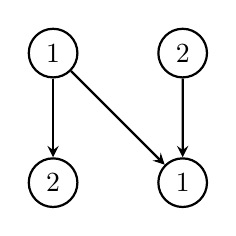
\begin{tikzpicture}[xscale=6,
yscale=8,>=stealth]
\tikzstyle{v}=[circle,
minimum size=1mm,draw,thick]
\node[v] (a) {$1$};
\node[v] (b) [right=of a] {$2$};
\node[v] (c) [below=of a] {$2$};
\node[v] (d) [below=of b] {$1$};
\draw[thick,->]
(a) to node {} (c);
\draw[thick,->]
(a) to node {} (d);
\draw[thick,->]
(b) to node {} (d);
\end{tikzpicture}








\end{document}